\documentclass[11pt]{article}

\usepackage{latexsym}
\usepackage{amsmath}
\usepackage{amssymb}
\usepackage{amsthm}
\usepackage{graphicx}
\usepackage{svg}
\usepackage{amsmath}
\graphicspath{ {images/} }
\usepackage{wrapfig}
\usepackage{pseudocode}
\usepackage{url}
\usepackage[backref, colorlinks=true, citecolor=red, urlcolor=blue, pdfauthor={Jyh-Ming Lien}]{hyperref}


\newcommand{\handout}[5]{
  \noindent
  \begin{center}
  \framebox{
    \vbox{
      \hbox to 5.78in { {\bf } \hfill #2 }
      \vspace{4mm}
      \hbox to 5.78in { {\Large \hfill #5  \hfill} }
      \vspace{2mm}
      \hbox to 5.78in { {\em #3 \hfill #4} }
    }
  }
  \end{center}
  \vspace*{4mm}
}

\newcommand{\lecture}[4]{\handout{#1}{#2}{#3}{#4}{#1}}

\newtheorem{theorem}{Theorem}
\newtheorem{corollary}[theorem]{Corollary}
\newtheorem{lemma}[theorem]{Lemma}
\newtheorem{observation}[theorem]{Observation}
\newtheorem{proposition}[theorem]{Proposition}
\newtheorem{definition}[theorem]{Definition}
\newtheorem{claim}[theorem]{Claim}
\newtheorem{fact}[theorem]{Fact}
\newtheorem{assumption}[theorem]{Assumption}

% 1-inch margins, from fullpage.sty by H.Partl, Version 2, Dec. 15, 1988.
\topmargin 0pt
\advance \topmargin by -\headheight
\advance \topmargin by -\headsep
\textheight 8.9in
\oddsidemargin 0pt
\evensidemargin \oddsidemargin
\marginparwidth 0.5in
\textwidth 6.5in

\parindent 0in
\parskip 1.5ex
%\renewcommand{\baselinestretch}{1.25}

\begin{document}

\lecture{Voronoi Stippling Report}{Fall 2017}{Yongxin Wang}{Advance Algorithm Programming}

\section{Summary of the two methods}
Given an input image, the two mothods both try to generate an image filled with stipples which resembles the input image. To do this, the hedcutter and voronoi methods are following the four steps as below.
\begin{enumerate}
  \item initialize sample points among the image, repeat from step2 to step4 until convergence
  \item create voronoi diagram using the sample ponits
  \item compute weighted centers for every voronoi region
  \item move each sample point to its corresponding center
\end{enumerate}
The difference between the hedcuter and voronoi methods are the different ways of generating voronoi diagram, which will be described in their individual sections. Then the two algorithms share the same procedure. In order to generate proper stipple image which resembles the original image, a method based the weighted centroidal voronoi diagram(CVT) is applied. In the process of computing weighted CVT, regions with higher values of ρ(a density function) will pack generating points closer than regions with lower values[1]. The proposed methods use color intensity from the input image as ρ, which in result packs more points around regions whose colors are closer to black while distributes fewer points around white regions. After several iterations this algorithm will generate an image with stipples which looks like the input image when configuration of parameters is good.
\subsection{hedcuter method}
% CVD : A centroidal Voronoi diagram has the interesting property that each generating point lies exactly on the centroid of its Voronoi region. 
% Lloyd’s method: (similar to K-means)
% weighted CVT
% Regions with higher values of ρ will pack generating points closer than regions with lower values
% do while(1,2,3)
% 1. build the VOR once. Image-based method
% propagate
% void CVT::vor(cv::Mat &  img)
% 2. weighted CVT, compute center
% 3. move the site to the center of its coverage
% inline float move_sites(cv::Mat & img, VorCell & cell)

The hedcuter method will compute voronoi diagram using the input image. The method is based on the property of voronoi diagram, which is that points inside the voronoi region is closer to its own site than all the other sites. For each sites, they propagate their labels to the four-connected neighbors and then those updated pixels will propagate labels to theirs neighbors and so on. This is processed in the manner of breadth-first search, which means at the end of each iteration every sites have reached out the same steps. Labels competing will happen when two sites have covered the same pixel and the site which is "closer" to such pixel will win. The hedcuter method will get the approximate voronoi diagram when there will be no update in terms of labels. The running time depends on three factors: the number of sites n; the resolution of the image (width, height) and the distribution of pixels. The lower bound is $O(width\times height)$ and the upper bound is $O(width\times height \times n)$.

\subsection{voronoi method}
% 1. build the VOR once(Fortune’s algorithm)
% 2. displacement towards center
% 3. move to center
The voronoi method uses Fortune's algorithm to generate voronoi diagram. Fortune's method is a sweep line algorithm and it can be computed in O(nlogn) time. 


\section{Comparison of the two methods}
%   speed, ouput, input, parameters
%0. hedcut is based on different metric measurement ???
%1. Do you get the same results by running the same program on the same image multiple times?
%2. If you vary the number of the disks in the output images, do these implementations produce the same distribution in the final image? If not, why?
%3. If you vary the number of the disks in the output images, is a method faster than the other?
%4. Does the size (number of pixels), image brightness or contrast of image increase or decrease their difference?
%5. Does the type of image (human vs. machine, natural vs. urban landscapes, photo vs. painting, etc) increase or decrease their difference?
%6. Are the outputs of these stippling methods different the hedcut images created by artists (e.g. those from the Wall Street Journal)?

\begin{enumerate}
  \item Output consistency: Voronoi method gives the same result every time given enough iteration, while hedcuter method's outputs vary. For the testing image, it seems that hedcuter will never converge using maximum distance termination condition, though it gives relatively good results after the first several iterations. The initial sample procedure and the number of iteration are factors of making the results differ from each other. They will affect the approximate voronoi diagram generated by hedcuter method.
  \begin{figure}[h!]
      \centering
      \subfloat[Hedcuter1]{{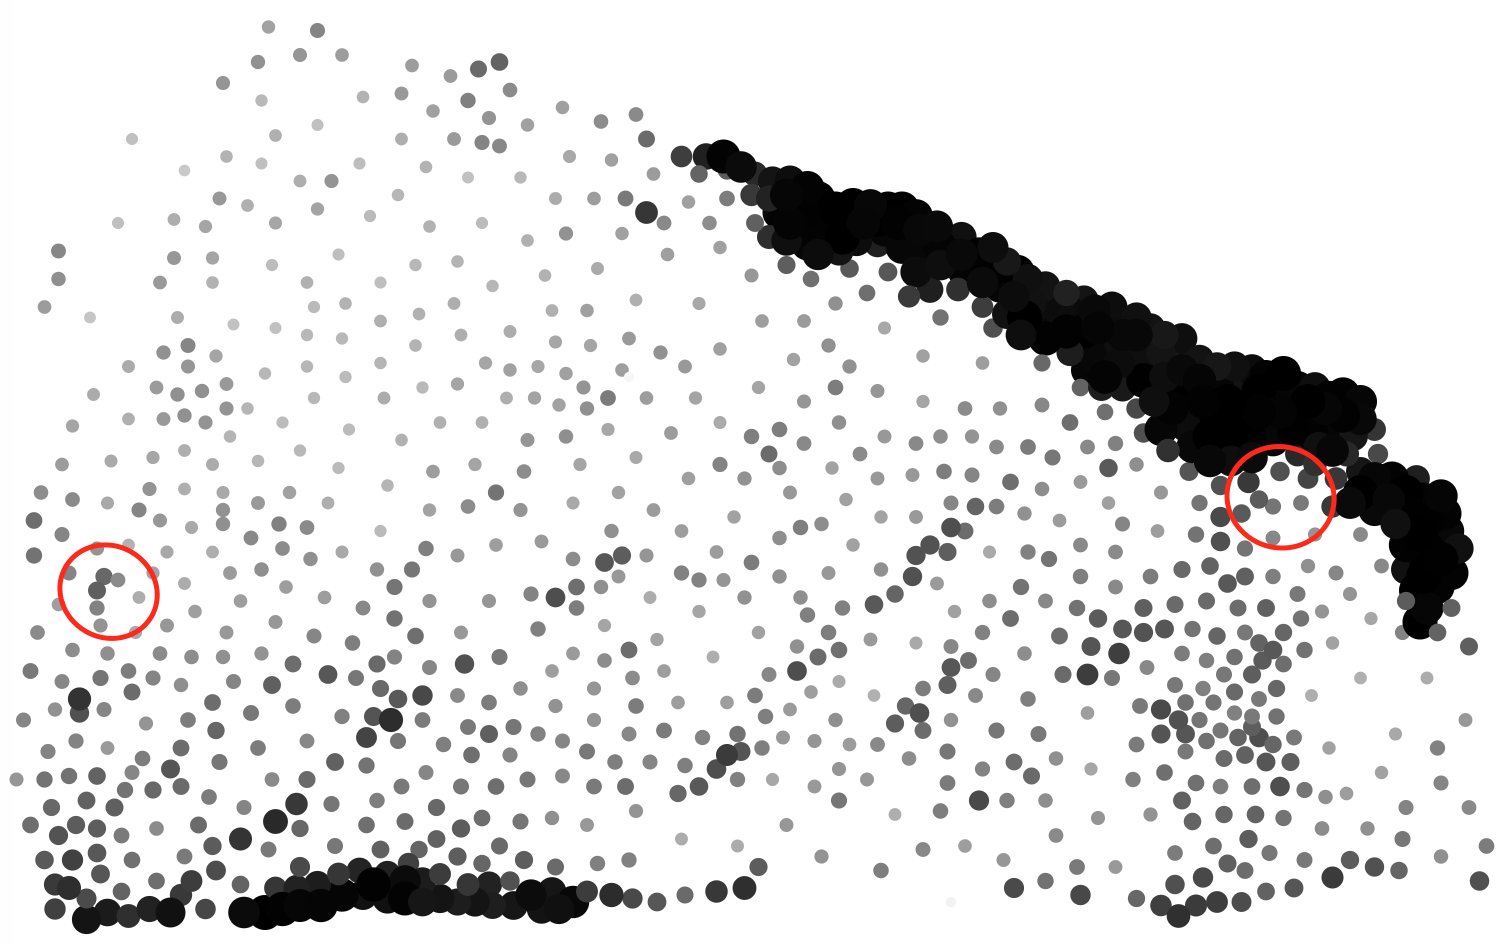
\includegraphics[width=5cm]{erinking-1000-1}}}
      \qquad
      \subfloat[Hedcuter2]{{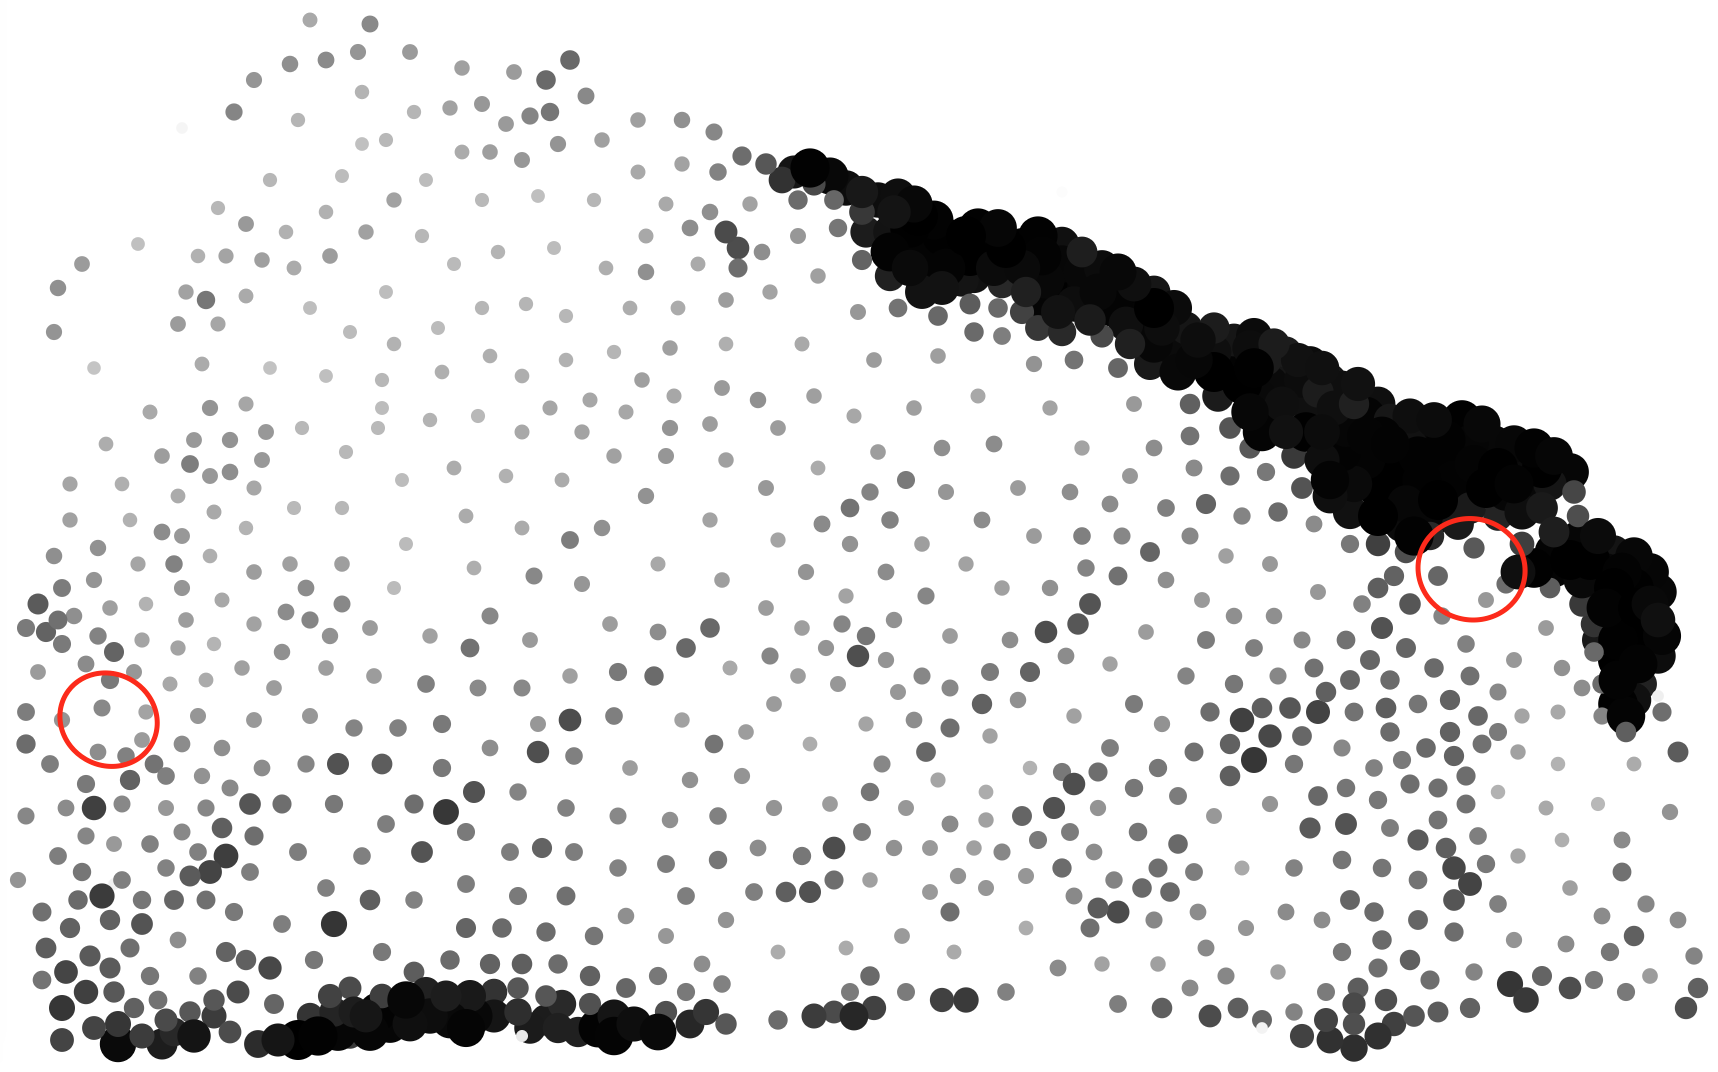
\includegraphics[width=5cm]{erinking-1000-2}}}
      \caption{Two results from Hedcuter on the same image}
      \label{fig:consistency}
  \end{figure}
  %2. If you vary the number of the disks in the output images, do these implementations produce the same distribution in the final image? If not, why?
  \item Distribution comparison. The distributions are not the same when the nubmer of the disk varies. When the number of disks drops, the voronoi's points evenly cover the image area while the hedcuter's points pack in the darker area. For the voronoi's method, the intensity information is easy to be filtered out when number of disks is low because there's a higher chance the intensity will be balanced out when the number of pixels in each region is high. While the hedcuter's method at the first step already takes intensity information into account. So they have different distribution when the number is low. Though when the number increases, the voronoi's method will focus on detailed region, where intensity information will take place.
  \begin{figure}[h!]
      \centering
      \subfloat[voronoi]{{
\includegraphics[width=5cm]{erinking-100-voronoi} }}
      \qquad
      \subfloat[hedcuter]{{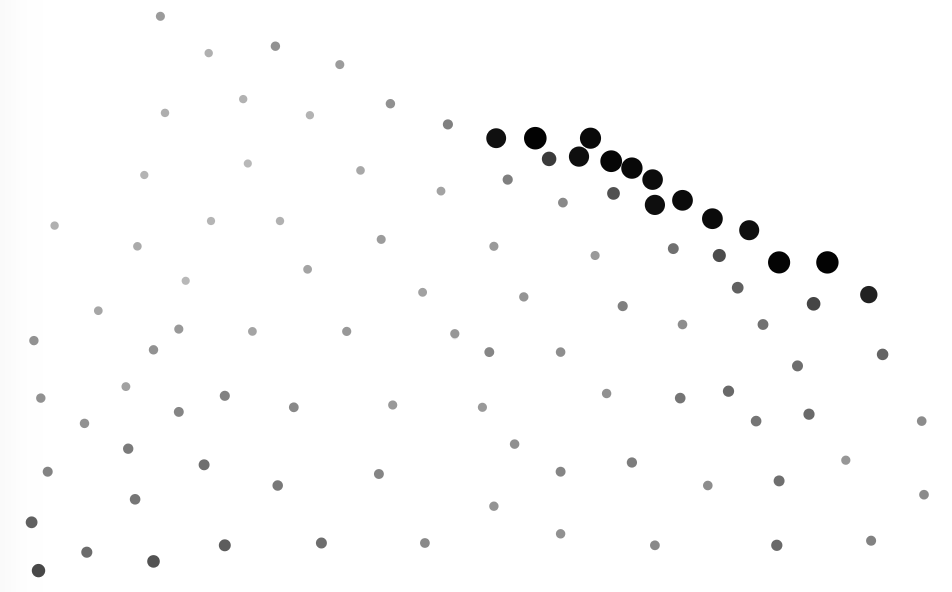
\includegraphics[width=5cm]{erinking-100-hedcuter} }}
      \caption{Left - voronoi's result; Right - hedcuter's result;}
      \label{fig:distribution}
  \end{figure}
  \newpage
  %3. If you vary the number of the disks in the output images, is a method faster than the other?
  \item Speed comparison. Voronoi method is faster than hedcuter method when number of the disks increases. The voronoi's method can compute voronoi diagram in O(nlogn) time, while the hedcuter's method has an upper bound as $O(width\times height \times n)$. When the number of disks is high, the hedcuter's method tends to move to its upper bound because the chance that one pixel is updated increases when the number is high.
  \begin{figure}[h!]
      \centering
      \subfloat[speed comparison]{{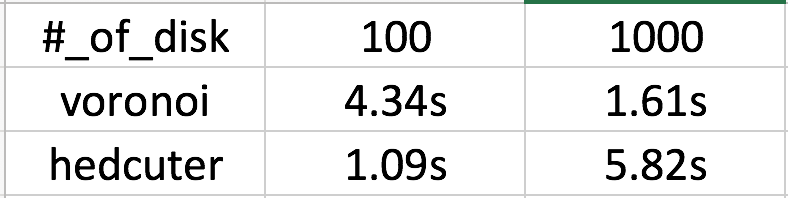
\includegraphics[width=5cm]{speed_comparison} }}
      \label{fig:speed}
  \end{figure}
  % table
  % 4.34s -> 1.61s
  % 1.09s -> 5.83s

  %4. Does the size (number of pixels), image brightness or contrast of image increase or decrease their difference?
  \item Their difference increases when the resolution of the image increases. When the resolution of the image is high, the hedcuter's method will capture more of the small\_region details of the original image because it can propagate the information out. Though the voronoi's method will balance such small\_region details with other sparse ares.
  \begin{figure}[h!]
      \centering
      \subfloat[voronoi-low-res]{{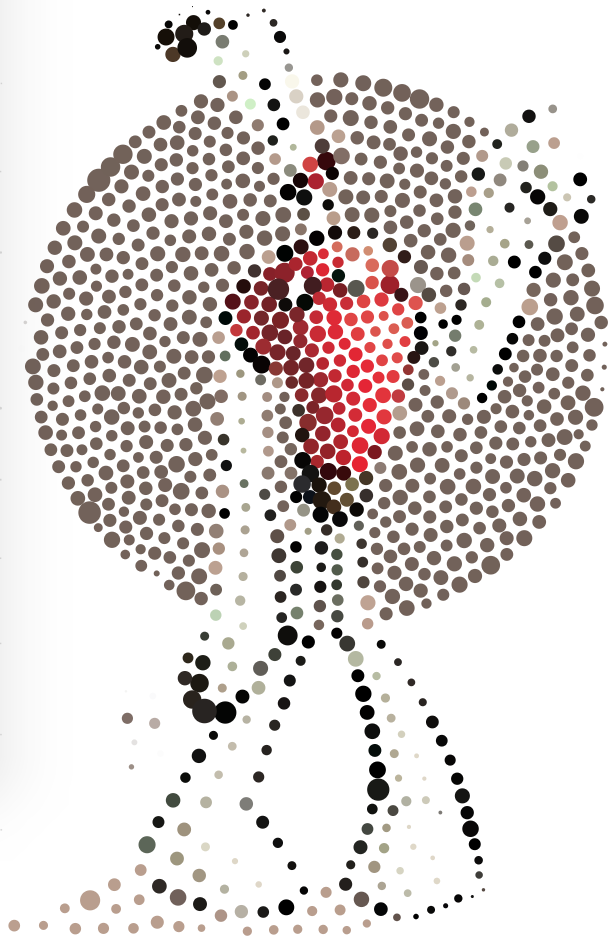
\includegraphics[width=3cm]{klaymen1-voronoi} }}
      \qquad
      \subfloat[voronoi-high-res]{{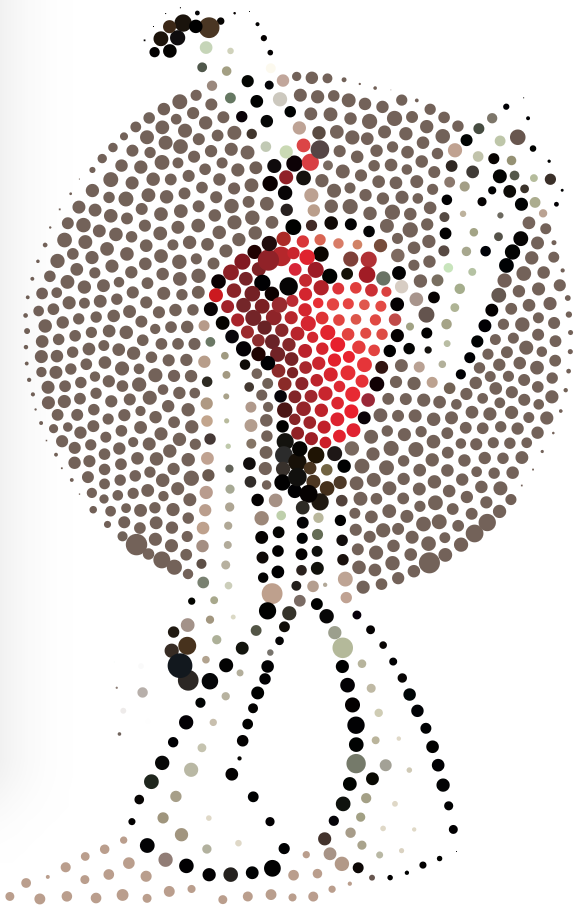
\includegraphics[width=3cm]{klaymen-voronoi} }}
      \qquad
      \subfloat[hedcuter-low-res]{{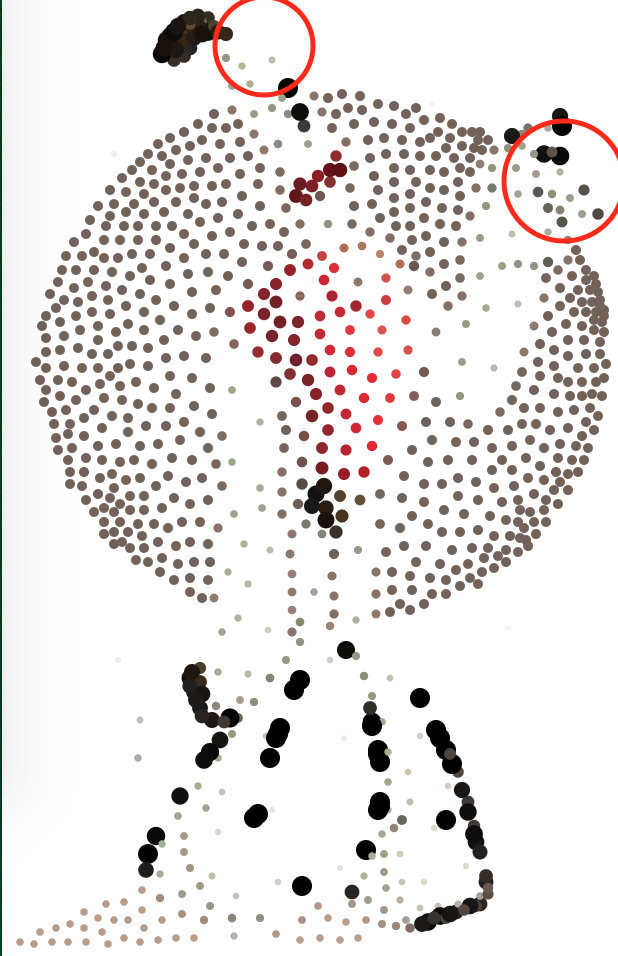
\includegraphics[width=3cm]{klaymen1-hedcuter} }}
      \qquad
      \subfloat[hedcuter-high-res]{{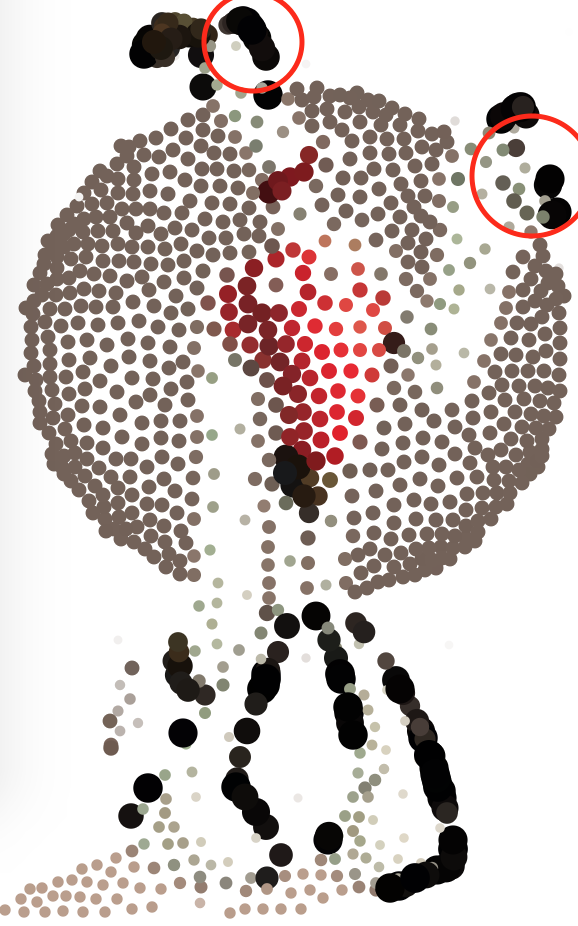
\includegraphics[width=3cm]{klaymen-hedcuter} }}
      \caption{resolution}
      \label{fig:klayman-hedcuter}
  \end{figure}
  % voronoi: 1.94s -> 10.09s
  % hedcuter: 5.47s -> 11.82s
  %6. Are the outputs of these stippling methods different from the hedcut images created by artists (e.g. those from the Wall Street Journal)?
  
  \item The outputs differ from the images created by artists. The artists uses lines instead of dots to represent line-property objects like hair and grid, while the program uses dots for all the objects. Also, the images created by the program have blurred borders.
  \begin{figure}[h!]
      \centering
      \subfloat[Artist]{{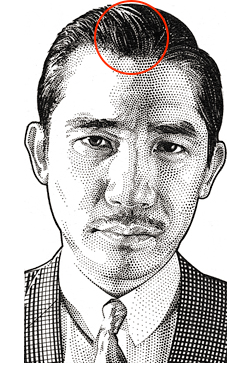
\includegraphics[width=3cm]{Liang_hedcut} }}
      \qquad
      \subfloat[Voronoi]{{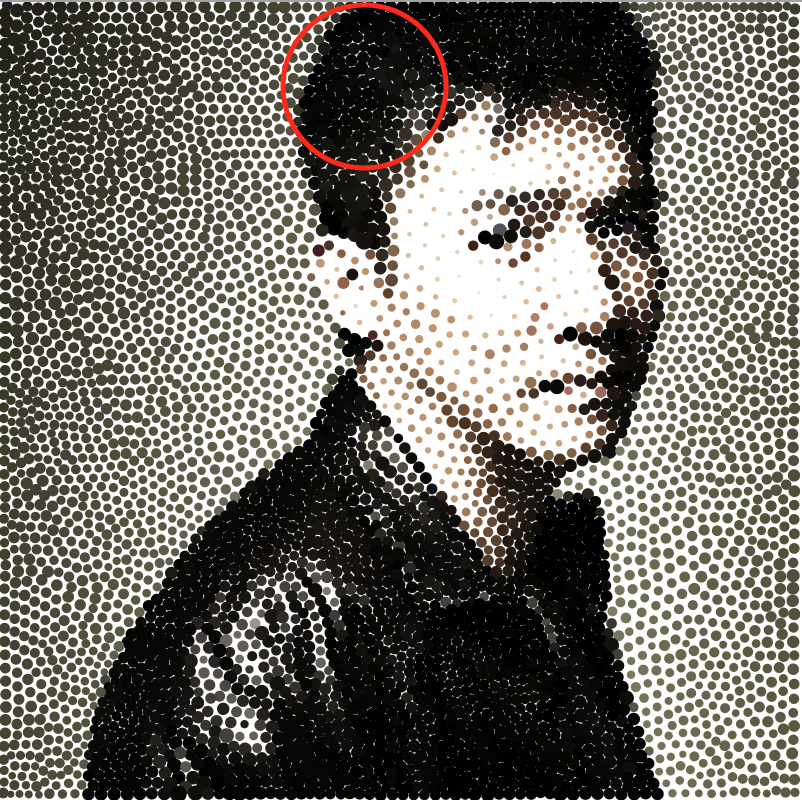
\includegraphics[width=4cm]{Liang-5000-voronoi} }}
      \qquad
      \subfloat[Hedcuter]{{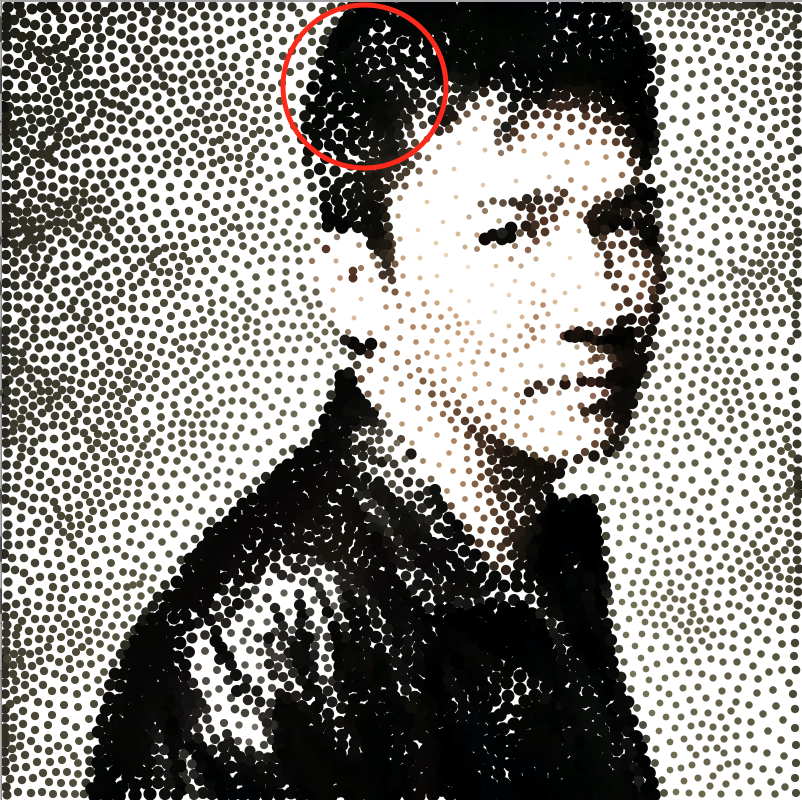
\includegraphics[width=4cm]{Liang-5000-hedcuter} }}
      \qquad
      \subfloat[Original]{{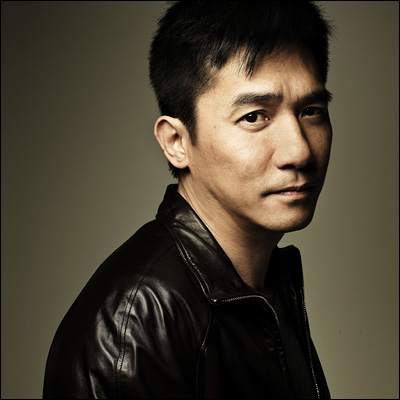
\includegraphics[width=2cm]{Liang_rgb} }}
      \caption{comparison with Wall Street Hedcut}
      \label{fig:klayman-hedcuter}
  \end{figure}
\end{enumerate}


\section{Improvement of hedcuter method}
\begin{enumerate}
  \item Decay. The program changes the propagation decay from $1.0$ to $0.5$, which leads to a more detailed representation of the original image. In the new method, the left eye shows up and the border of the head also becomes less blurred. When the decay rate is applied to propagation, the effect of the cell on farther pixels decreases. This in result makes the cell less involved with others and the details show up.
  \begin{figure}[h!]
      \centering
      \subfloat[decay: 1.5]{{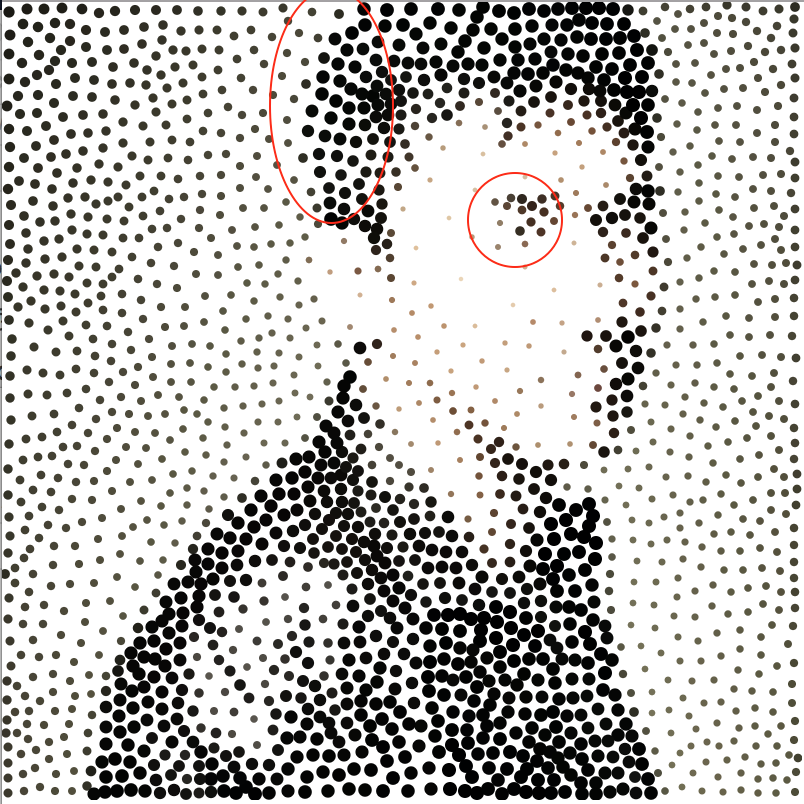
\includegraphics[width=4.5cm]{decay-1-5} }}
      \qquad
      \subfloat[decay: 1.0]{{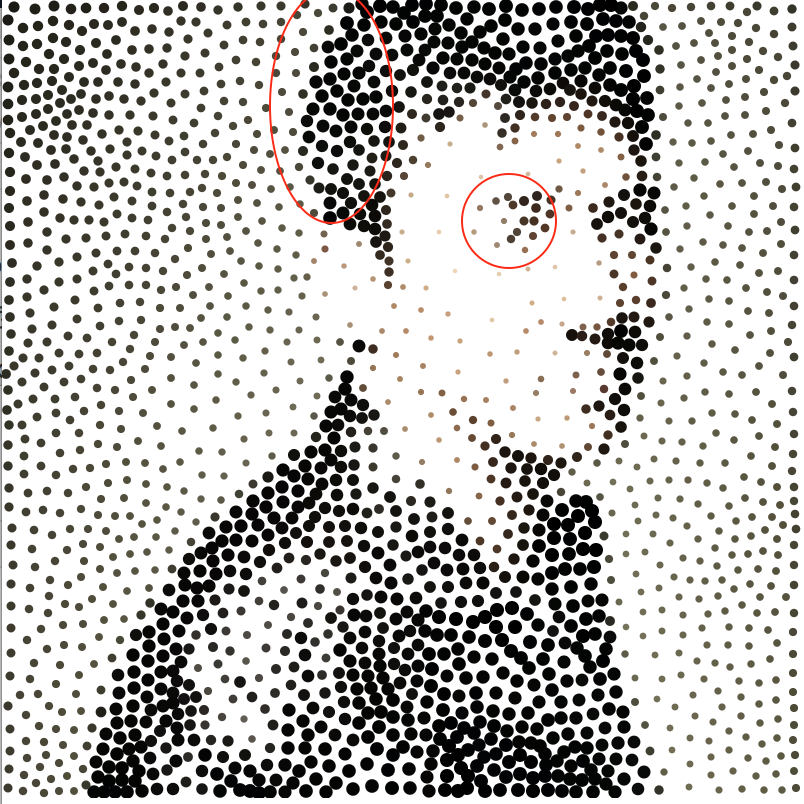
\includegraphics[width=4.5cm]{decay-1-0} }}
      \qquad
      \subfloat[decay: 0.5]{{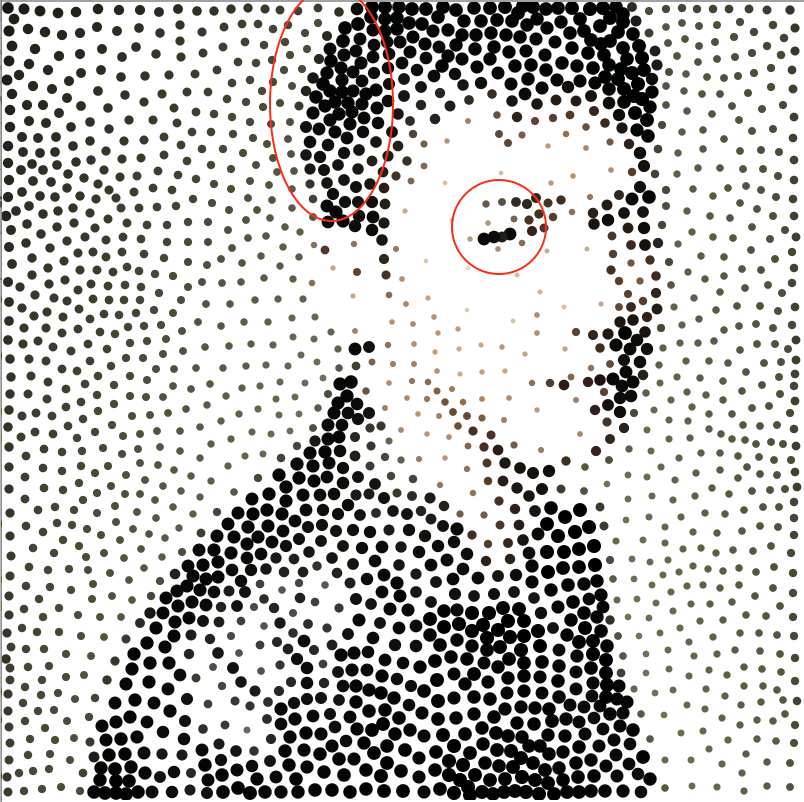
\includegraphics[width=4.5cm]{decay-0-5} }}
      \caption{Decay Demonstration}
      \label{fig:Liang-decay}
  \end{figure}
  \item Pre-compute grid. This method uses the precompute method in the suggested paper, which construct the dot image by concatenate several 20-by-20 small dot images. The density of the small image is decided by the average image intenstiy in the corresponding image block in the input image.
  \begin{figure}[h!]
      \centering
      \subfloat[gray image]{{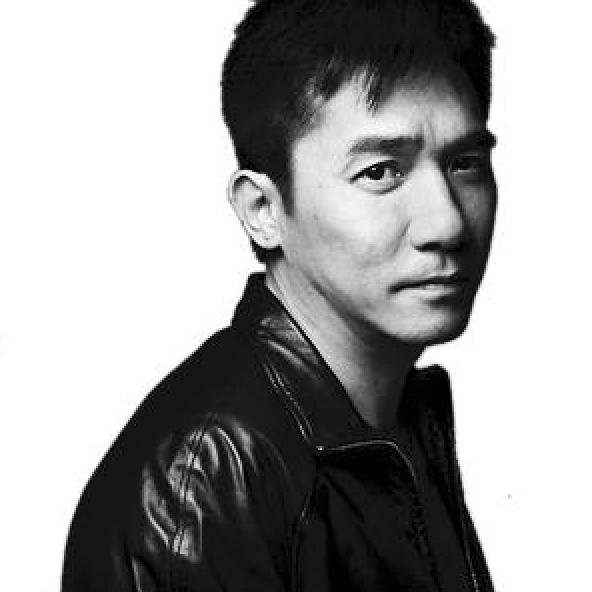
\includegraphics[width=4cm]{Liang-gray1} }}
      \qquad
      \subfloat[hedcut: 1500]{{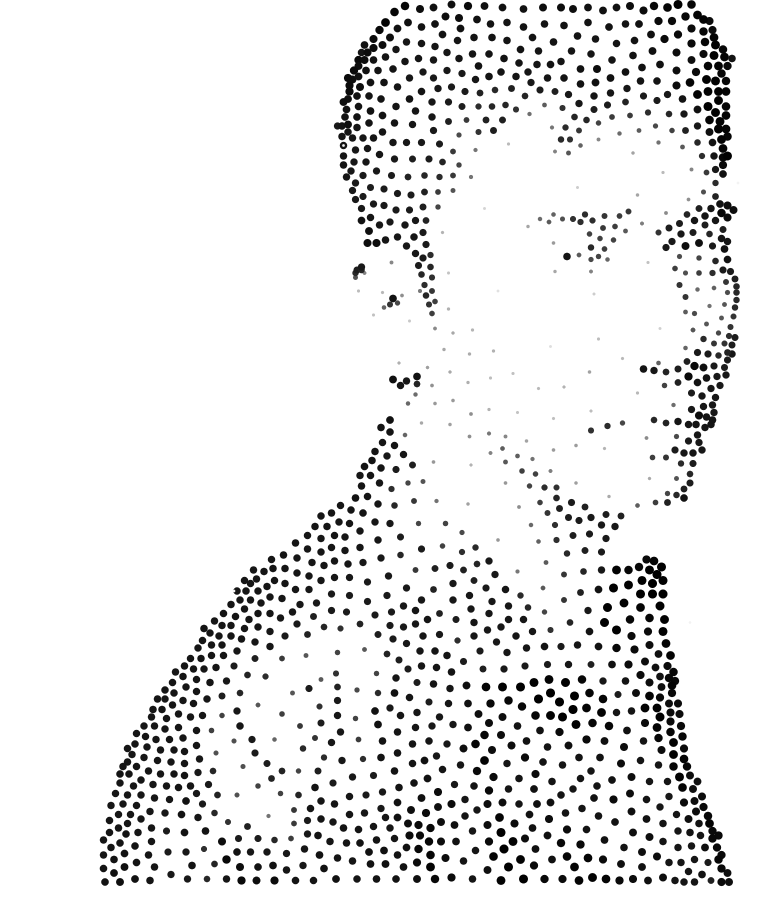
\includegraphics[width=4cm]{Liang-gray1-hedcut} }}
      \qquad
      \subfloat[precompute]{{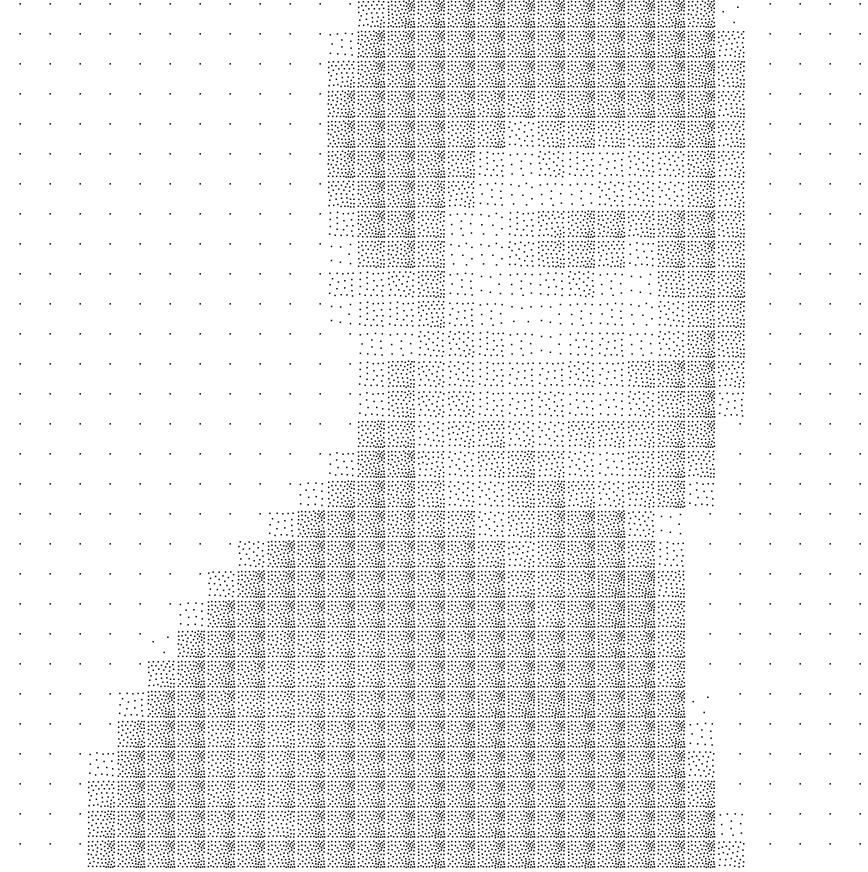
\includegraphics[width=6cm]{Liang-gray1-precompute} }}
      \caption{Precompute grid}
      \label{fig:Liang-precompute}
  \end{figure}
  % edge-detection + orignal input: how to combine the two results?
  \newpage
  \item Edge based hedcuter. The results in section2 show the weakness of hedcuter on discriminate between edges and non-edges. The proposed method thus makes an attempt to utilize the outcomes of canny edge detection. By putting more weight on non-edge pixels, the method appears to make some improvements on enhancing the visibility of edges on the examples below. The two lines circled in the final result(Right) shows the edges in the canny result(Left) that were not captured using hedcuter method(Middle) due to the closeness of intensity in the neighborhood.
  \begin{figure}[h!]
      \centering
      \subfloat[edge detection]{{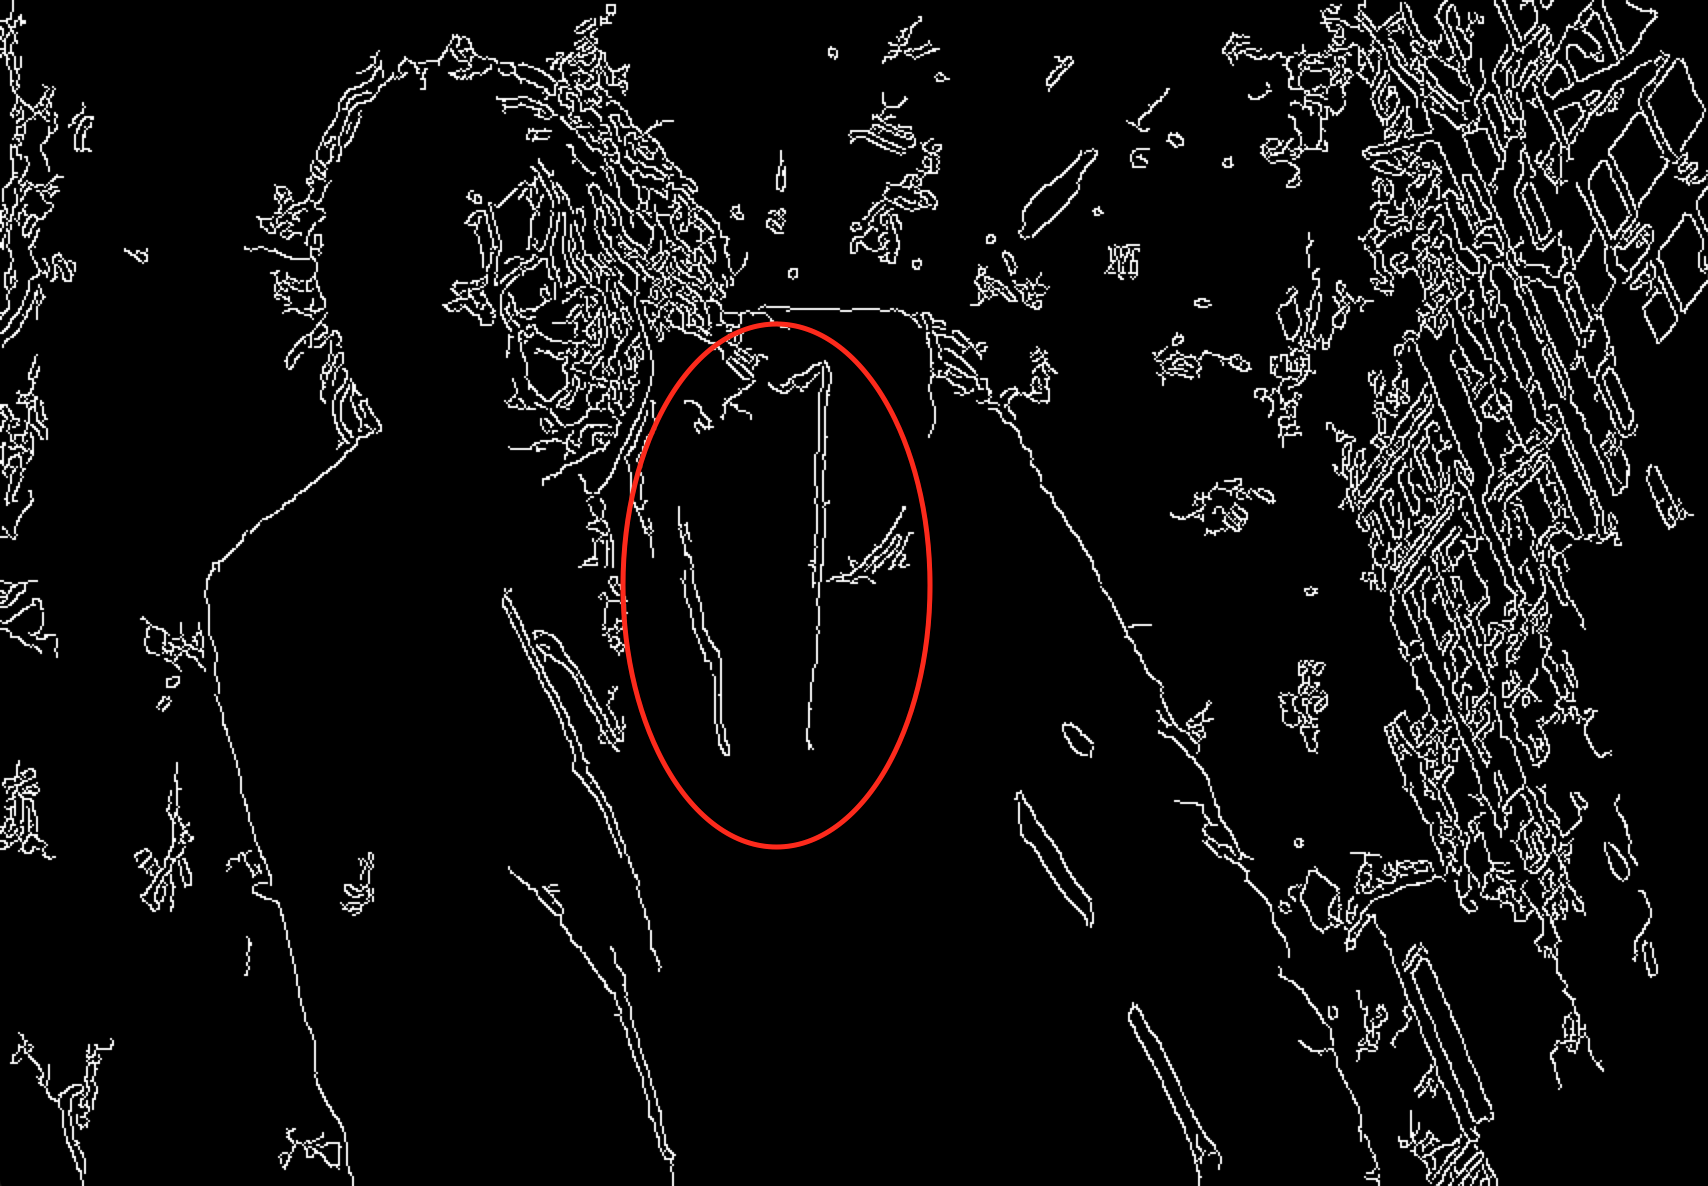
\includegraphics[width=4.5cm]{canny} }}
      \qquad
      \subfloat[hedcut]{{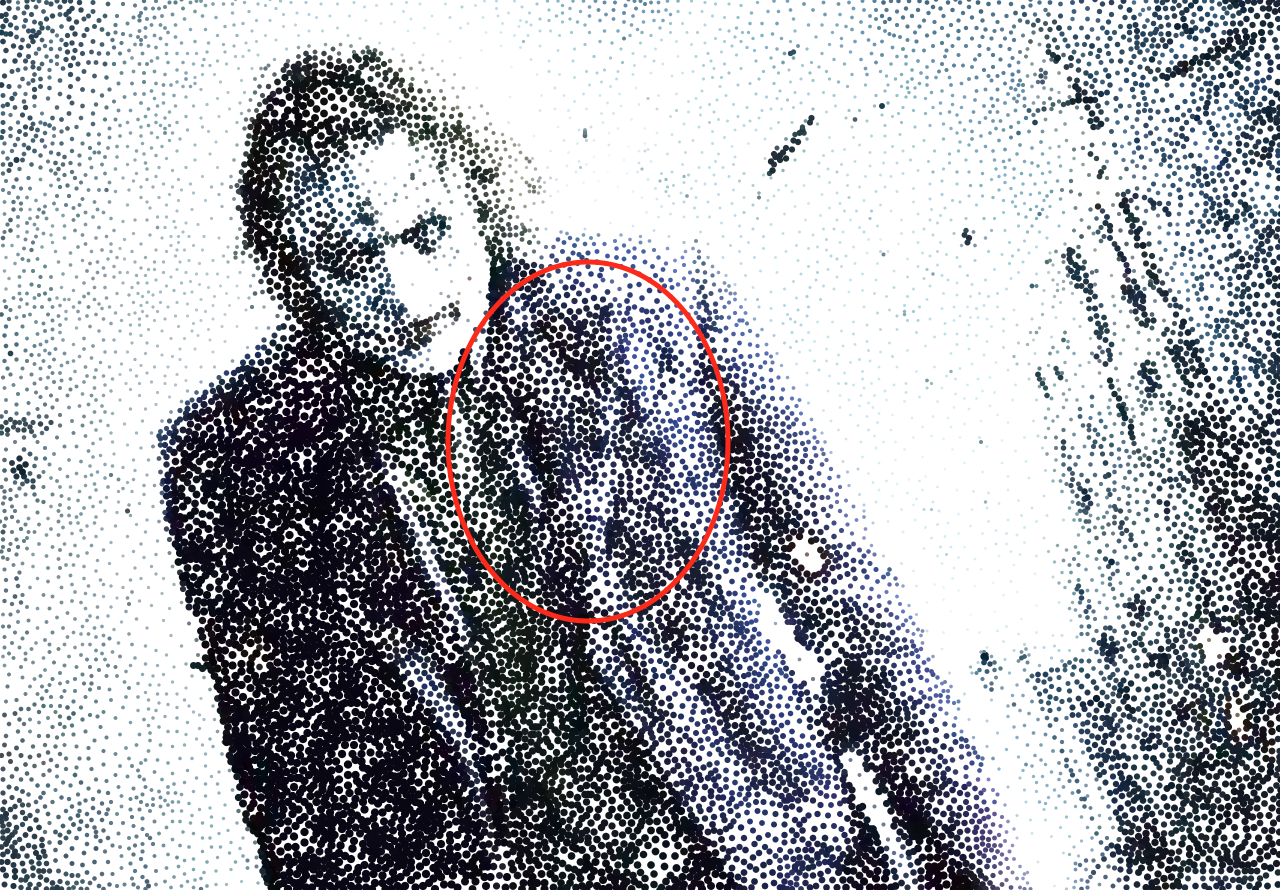
\includegraphics[width=4.5cm]{joker-hedcut} }}
      \qquad
      \subfloat[hedcut+edge]{{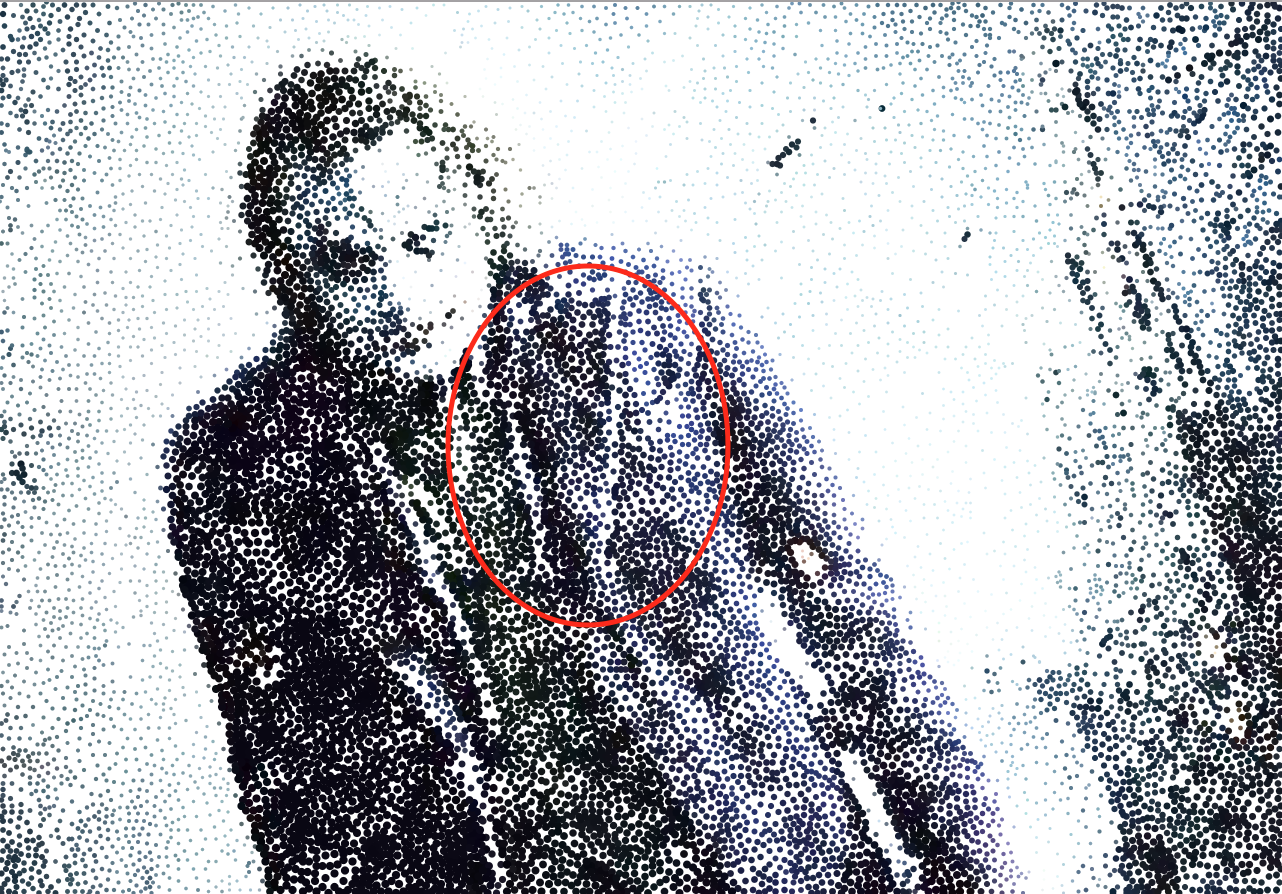
\includegraphics[width=4.5cm]{joker-edge2} }}
      \caption{edge-present hedcuter}
      \label{fig:Liang-edge}
  \end{figure}

  
\end{enumerate}

% 2. border : 
% 3. pre-compute : 
% 4. 

\bibliographystyle{plain}
\bibliography{report}

\end{document}


